\newpage
\section{Priors, Regularization, AIC, BIC, LRT}

Every time we increase the complexity of our model, for a fixed data set, its Maximum Likelihood fitting accuracy increases. While this trend seems encouraging, it is desired only up to a certain point, after which the model starts adapting to the idiosyncrasies of the data while becoming insensitive to its features that are truly generalizable. The resulting a fitted model will work very well for the data at hand, but under-perform on similar but slightly different future data. This is ``overfitting''.

Since models, being a mathematical constructs, cannot tell the difference between generalizable features and noise in the data, we need to guide them by providing additional information. We need to come to terms with our own expectations (based on intuition or historical data) and turn them into mathematical requirements. Priors and regularization, and model selection via various information criteria are common ways.


\subsection{Improper and proper priors}
\no Improper priors are not normalizable, i.e. $\sum_\theta P(\theta) = \infty$. Examples are
\begin{itemize}
	\item Flat priors: $P(\theta) = \text{const.}$ over any infinite domain.
	\item ``Uninformative'' priors, which are usually derived from transformation invariance or max-entropy principles:
	\begin{itemize}
		\item Location parameter: $P(m) = \text{const.}$, on $m \in (-\infty, +\infty)$,
		\item Scale parameter: $P(s) = \frac{\text{const.}}{s}$, on $s\in (0, \infty)$,
		\item Probability parameter: $P(p) = \frac{\text{const.}}{p(1-p)}$, on $p\in(0,1)$.
	\end{itemize}
	\item ``Reference priors'' that maximize the sensitivity of the inference of one selected model parameter.
	\item Jeffrey's priors for certain models, which equalizes the Fisher information on the parameter space, e.g. $P(\sigma^2) = 1 / \sigma^2$ for the Normal model.
\end{itemize}
Priors that are normalized are proper priors, i.e. $\sum_\theta P(\theta) = 1$. Examples are
\begin{itemize}
	\item Distributions with carefully chosen parameter values, e.g. $\text{Beta}(\theta\;|\;\alpha = 1,\beta = 1)$
	\item Jeffrey's priors for certain models, e.g. $P(p) = \frac{1}{\pi\sqrt{p (1-p)}}$ for Bernoulli model (or Binomial model).
\end{itemize}
Note: A prior (proper or improper) $P(\theta)$ can be used in the Maximum Likelihood Estimation context by adding their logarithm to the log likelihood function $L(\theta)$ before maximizing,
\be
	\theta_\text{MLE} = \amax_\theta L(\theta)
	\qquad \rightarrow \qquad
	\theta_\text{MAP} = \amax_\theta \Big[ L(\theta)  + \log P(\theta)\Big],
\ee
yielding the ``maximum a posteriori'' estimate, in other words, the mode of the posterior distribution.

\subsection{Regularization}
\no Regularization is a general process during which we add a data-independent term to the (data-dependent) cost function before minimizing it.
\begin{itemize}
	\item We collect data $D$, 
	\item specify a model $M$ with parameters $\theta$, and log likelihood $L(\theta) = \log P(D\;|\;\theta)$.
	\item The cost function is usually derived directly from the log likelihood: $\text{cost}(\theta, D) = - L(\theta)$, but some models define the cost function directly without referencing statistical models.
	\item We introduce a penalty term $\text{penalty}(\theta)$ that is high for implausible $\theta$ values,
	\item and minimizes the regularized cost to obtain the regularized optimum $\theta_\text{reg,opt}$,
	\be
		\theta_\text{reg,opt} = \text{arg min}_\theta (\text{cost}(\theta, D) + \text{penalty}(\theta))
	\ee
\end{itemize}

\subsection{Linear regression}
Linear regression is the simplest model where number of model parameter can be systematically increased without bounds. (Once one runs out of raw features, $x_{.,k}$, interactions binary, and higher order, interactions features, e.g. $x_{.,k} x_{.,l}$.) Let's see how regularization is used to guide model fitting.

\begin{itemize}
	\item The process start by recording $K$ features and one ``outcome'' variable for each of the $N$ observations. This results in the data set $D = \{\;(\{x_{i,k}\}_{k=1}^K, \;y_i)\;\}_{i=1}^N$, where $x_i\in \mathds{R}^K$ is a feature vector and $y_i \in \mathds{R}$ is the outcome variable that we wish the model to predict.
	\item The linear model 
	\begin{itemize}
		\item aims to predict the outcome $y$ by linearly combining the $K$ components of the feature vector $x$. For this, the model needs $K$ coefficients (or weights) $b = \{b_k\}_{k=1}^K \in \mathds{R}^K$.
		\item The noise is often modeled as one dimensional normal distribution along $y$ with unknown variance.
		\item These two consideration result in the following three (identical) formulation of the model:
		\ba
			y_i &=& \sum_{k=1}^K x_{i,k} b_k + \varepsilon_i, \quad \text{with}\quad P(\varepsilon_i) = \text{Normal}(\varepsilon_i\;|\; \mu = 0, \sigma^2 = \sigma^2) \\
			&& \text{or, equivalently} \\
			y &=& X b + \varepsilon,\quad \text{with}\quad P(\varepsilon) = \text{Multi-variate-normal}(\varepsilon\;|\;\mu = 0, \Sigma = \mathds{I} \sigma^2) \\
			&& \text{or, equivalently} \\
			P(y\;|\;X, b, \sigma^2) &=& \prod_{i=1}^N\text{Normal}\left(y_i\;\big|\;\mu = (X b)_i, \;\sigma^2=\sigma^2\right)
		\ea
		where $X$ is a matrix of features, also called the ``design matrx'', whose elements are $X_{i,k} = x_{i,k}$, and the product between $X$ and $b$ is understood to be matrix multiplication, i.e. $(Xb)_i = \sum_k x_{i,k} b_k$. The symbol $\mathds{I}$ inside the argument of the multi-variate normal distribution is the $K$-dimensional identity matrix.
	\end{itemize}
	\item Using the formula of the normal distribution, the log likelihood can be written as
	\be 
		L(b, \sigma^2) = \log P(y\;|\;X, b, \sigma^2) = -\frac{N}{2}\log(\sigma^2) - \frac{1}{2\sigma^2} \sum_{i=1}^N \Big[y_i - \sum_{k} x_{i,k} b_k\Big]^2
	\ee
	Taking the partial derivatives with respect to $b_k$ (and $\sigma^2$), setting them to zero and solving the system of equations yields the (non-regularized) maximum likelihood estimates 
	\be
		b_\text{MLE} = \text{arg max}_b\; L(b, \sigma^2) = (X^\top X)^{-1} X^\top y, \qquad (\sigma^2)_\text{MLE} = \frac{1}{N}|| y - Xb ||^2,
	\ee
	where $X\T$ is the transpose of $X$, i.e. $(X\T)_{k,i} = x_{i,k}$, and $(X\T X)_{k,l} = \sum_i x_{i,k}x_{i,l}$, and $(X\T y)_k =  \sum_i x_{i,k} y_i$. The operator $||.||$ stands for the $L_2$ norm of a vector, in other words, its Euclidean length: $||y|| = \sqrt{\sum_{i} y_i^2}$.

	\item The three most commonly used regularization methods are 
	\begin{itemize}
		\item ``L1 regularization'', which tries to keep the total absolute sum of the coefficients low using a penalty term that is equivalent to specifying Laplace prior for each $b_k$,
		\be
			\text{penalty}(b) = \alpha_1 \sum_k |b_k|\qquad \Leftrightarrow \qquad P(b_k) = \text{const.} \times e^{- \alpha_1|b_k|} = \text{Laplace}(b_k\;|\;\text{loc}=0, \text{scale}=1/\alpha_1)
		\ee

		\item ``L2 regularization'', which tries to keep the total Euclidean length of the coefficient vector low using a penalty term that is equivalent to specifying normal prior for each $b_k$,
		\be
			\text{penalty}(b) = \frac{\alpha_2}{2}\sum_k (b_k)^2
			\qquad \Leftrightarrow \qquad
			P(b_k) = \text{const.} \times e^{- \alpha_2(b_k)^2 / 2} = \text{Normal}(b_k\;|\;\mu=0, \sigma^2=1/\alpha_2)
		\ee
		\item ``Elastic net'' regularization, which combines L1 and L2 regularization with adjustable weights $\alpha_1, \alpha_2$, 
		\be
			\text{penalty}(b) = \alpha_1 \sum_k |b_k| + \frac{\alpha_2}{2}\sum_k (b_k)^2
		\ee
	\end{itemize}
	In all three cases the ``hyperparameters'' $\alpha_1$ and $\alpha_2$ are often optimized using Leave-one-out or M-fold cross-validation. 

	\item Note: A fully Bayesian treatment of regularized models can be carried out by treating the hyperparameters as just another set of model parameters, and determine their posterior (usually numerically).
\end{itemize}

\subsection{Model comparison with asymptotic metrics}

In the maximum likelihood estimation context, when models with different set of parameters are fitted to the same data set, we often wish to determine which model has a better potential to generalize to future similar data sets. While some form of regularization (e.g. L1) is able to pick out important model parameters from unimportant ones, we need a different framework when comparing models with completely different structures. 

Asymptotic metrics, such as AIC, BIC, LRT p-value are useful for this analysis. Model selection methods based on these metrics, as their name suggests, are reliable only if we are close to the asymptotic limit of infinite data. In practice this requires us to have significantly more observations than model parameters.

Consider the general maximum likelihood fits of two models:
\begin{itemize}
	\item We focus on a fixed dataset $D = \{x_i\}_{i=1}^N$, and specify two models.
	\item One model, of lower complexity, is often called the ``null model'', $M_0$ with 
	\begin{itemize}
		\item parameters $\theta_0$,
		\item log likelihood $L_0(\theta_0) = \log P(D\;|\;\theta_0, M_0)$, and
		\item MLE fit $\theta_{0, \text{MLE}} = \text{argmax}_{\theta_0} L_0(\theta_0)$.
	\end{itemize}
	\item Another model, of higher complexity, is often called ``alternate model'', $M_1$ with 
	\begin{itemize}
		\item parameters $\theta_1$,
		\item log likelihood $L_1(\theta_1) = \log P(D\;|\;\theta_1, M_1)$, and
		\item MLE fit $\theta_{1, \text{MLE}} = \text{argmax}_{\theta_1} L_1(\theta_1)$.
	\end{itemize}
\end{itemize}
{\bf Akaike Information Criterion (AIC):} This method corrects the log likelihood with the number of parameters $\text{dim}(\theta)$ before comparison.
\begin{itemize}
	\item $\text{AIC}(M_i) := -2\Big[L_i(\theta_{i,\text{MLE}}) - \text{dim}(\theta_i)\Big]$ for both $i=0, 1$ models.
	\item If $\text{AIC}(M_1) < \text{AIC}(M_0)$, then $M_1$  is more plausible.
\end{itemize}
{\bf Bayesian Information Criterion (BIC):} This methods corrects the log likelihood with the number of parameter weighted by the logarithm of the total number of observations. It is considered more robust than AIC.
\begin{itemize}
	\item $\text{BIC}(M_i) := -2\left[L_i(\theta_{i,\text{MLE}}) - \frac{\ln(N)}{2}\text{dim}(\theta_i)\right]$ for both $i=0, 1$ models.
	\item If $\text{BIC}(M_1) < \text{BIC}(M_0)$, then $M_1$  is more plausible.
\end{itemize}
{\bf Likelihood Ratio Test (LRT):} If the null model is a restricted version of the alternate model (``nested models''), the likelihood ratio test determine if the extension from the null model to the alternate model increases the likelihood more than expected by random noise in the null model.
\begin{itemize}
	\item First, we calculate the log likelihood ratio, $\text{logLR} := \log\frac{P(D\;|\;M_1, \theta_{1,\text{MLE}})}{P(D\;|\;M_0, \theta_{0,\text{MLE}})} = L_1(\theta_{1,\text{MLE}}) - L_0(\theta_{0,\text{MLE}})$
	\item We expect $\text{logLR} > 0$, otherwise the null model is unquestionably superior.
	\item We calculate $\text{LRT p-value} := 1 - \text{cdf }\chi^2\Big(2\,\text{logRL}\;\Big|\;\text{dof} = \text{dim}(\theta_1) - \text{dim}(\theta_0)\Big)$, where $\text{cdf }\chi^2(\ldots\;|\;\text{dof}=d)$ is the cumulative distribution function of the $\chi^2$ distribution with degrees of freedom $d$.
	\item A small enough p-value, the threshold of which depends on how big false positive rate we can stomach, indicates that $M_1$ is more plausible than $M_0$.
\end{itemize}
{\bf Model evidence:} Using the either of the information criteria (IC), we can approximate the evidence for a model.
\begin{itemize}
	\item The evidence for model $M_i$ is $P(D\;|\;M_i) = \sum_{\theta_i} P(D\;|\;\theta_i, M_i) \approx \exp\left(-\frac{1}{2} \text{ IC}\right)$, 
	\item where IC can be either AIC or BIC (or WAIC, WBIC)
	\item Under uniform prior on the models (i.e. $P(M_0) = P(M_1)$), the posterior probability of the alternate model being correct is
		\be
			 P(M_1\;|\;D) \approx \frac{\exp\left(-\frac{1}{2} \text{ IC}_1\right)}{\exp\left(-\frac{1}{2} \text{ IC}_0\right) + \exp\left(-\frac{1}{2} \text{ IC}_1\right)}
		\ee
\end{itemize}

\newpage
\subsection{Example: Linear regression}
\no Let's see how the asymptotic metrics described above work for a simple liner regression problem.
\begin{itemize}
	
	\item We generate data: $D = \{(x_i, y_i)\}_{i=1}^N$, from the distribution $y = 1 - 3x - x^2/2 + x^3 + \varepsilon$ with $\text{std}(\varepsilon) = 2$).
\begin{lstlisting}[language=python]
import numpy as np
from numpy.polynomial.polynomial import polyval
from scipy.stats import norm

c_true = [1, -3, -0.5, 1]
sigma_true = 2
x_data = np.linspace(-3, 3, 20)
y_data = [polyval(x, c_true) + norm.rvs(loc=0, scale=sigma_true) 
          for x in x_data]
\end{lstlisting}
	\begin{figure}[h]
		\centering
		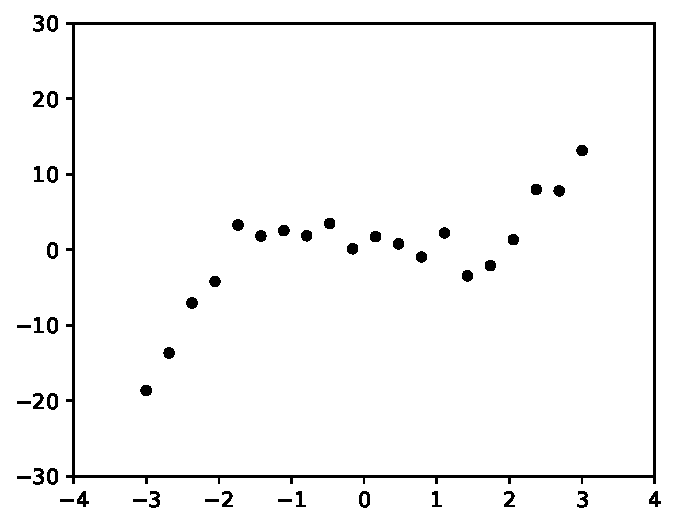
\includegraphics[width=0.45\textwidth]{./figs/03-linear-regression-data.pdf}
	\end{figure}
	
	\item Let's consider a series of models: $M_K$, where $K=0,1,2,\ldots 11$ indicates the degree of the polynomial for the ``main curve''. For each model $M_K$ the parameter vector is $c = (c_0, c_1, \ldots c_K) \in \mathds{R}^{K+1}$.
	
	\item Linear features vector is $X_i := (1, x_i, (x_i)^2, (x_i)^3),\ldots (x_i)^K) \in \mathds{R}^{K+1}$.
\begin{lstlisting}[language=python]
def generate_polynomial_features(x_data, degree):
    K = degree
    N = len(x_data)
    X = np.zeros([N, K+1])
    for i, x in enumerate(x_data):
        for k in range(0, K+1, 1):
            X[i,k] = x**k
    return X
\end{lstlisting}

	\item The log likelihood for the model
	$y = \sum_{k=0}^K X_{i,k} c_k  + \varepsilon$, with $P(\varepsilon) = \text{Normal}(\varepsilon \;|\; 0, \sigma^2)$, is $L(c) = \sum_i\log\Big( \text{Normal}(y_i\;|\; \mu = (Xc)_i, \sigma^2 = \sigma^2)\Big)$
\begin{lstlisting}[language=python]
def log_likelihood(X, y, c, sigma2):
    N = len(y_data)
    log_like = 0
    log_like += - N/2.0 * np.log(sigma2)
    log_like += - 1.0/(2 * sigma2) * vector_norm(y - X.dot(c))**2
    return log_like
\end{lstlisting}

	\item We calculate the MLE solution using the formulas $c_\text{MLE}= (X^\top X)^{-1} X^\top y$, \quad $(\sigma^2)_\text{MLE} = \frac{1}{N}||y - X c_\text{MLE}||^2$,
\begin{lstlisting}[language=python]
def fit_MLE_ploynomial(X, y):
    c_MLE = inv(X.T.dot(X)).dot(X.T).dot(y_data)
    sigma2_MLE = 1.0/len(y) * vector_norm(y - X.dot(c_MLE))**2
    return c_MLE, sigma2_MLE
\end{lstlisting}
 	We plot the fits on top of the data below, where the solid curve shows the mean of the prediction $y$ as a function of $x$, and the shaded region around it indicates the $2\sigma$ vertical interval around it. Visualizing this way and checking that $\sim 97.5\%$ (19-20) of the data points is covered by the shaded region allows us to verify that all fits are consistent with the data. 
	\begin{figure}[h]
		\centering
		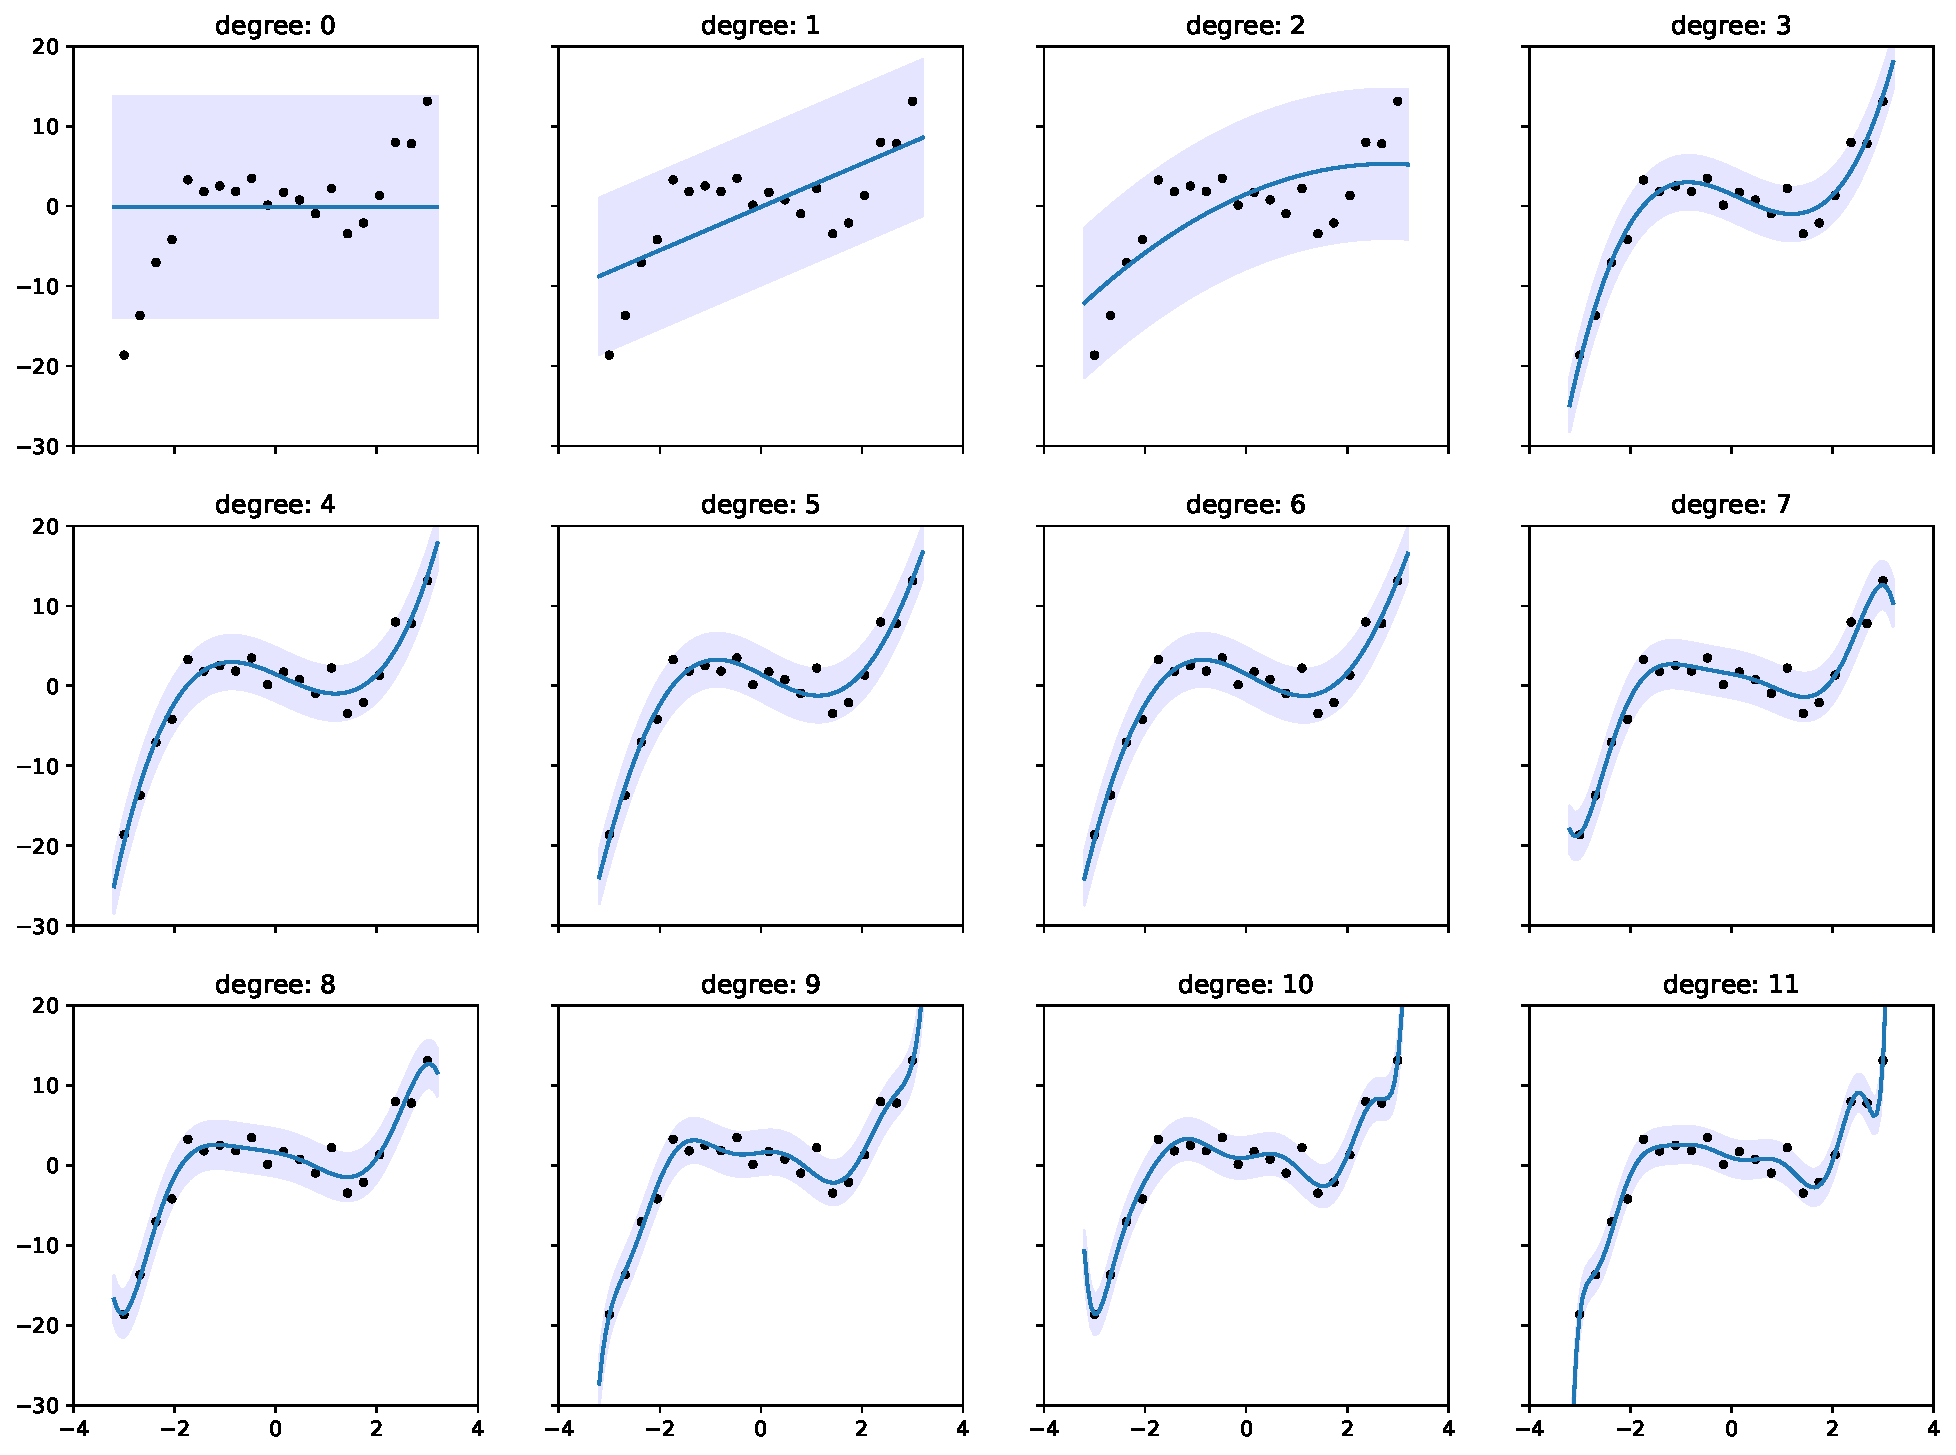
\includegraphics[width=\textwidth]{./figs/03-linear-regression-fits.pdf}
	\end{figure}

\end{itemize}

\newpage
\no Let's compare the different models $M_0, M_1, M_2\ldots M_{11}$ using AIC, BIC, likelihood ratio test.
\begin{itemize}
	\item AIC for model $M_K$ is $\text{AIC}_K = -2 [L_K - (K+2)]$, where $K+2 = \text{dim}(c, \sigma^2) =  \text{dim}(c) + \text{dim}(\sigma^2) = (K+1) + 1$, and $L_K$ is the maximal likelihood achievable with with model $M_K$.
\begin{lstlisting}[language=python]
def AIC(X, y, c, sigma2):
	dim = len(c) + 1
	loglike = log_likelihood(X, y, c, sigma2)
	return -2 * (loglike - dim)
\end{lstlisting}

	\item BIC for model $M_K$ is $\text{BIC}_K = -2 [L_K - \frac{\ln N}{2}(K+2)]$
\begin{lstlisting}[language=python]
def BIC(X, y, c, sigma2):
	N = len(y)
	dim = len(c) + 1
	loglike = log_likelihood(X, y, c, sigma2)
	return -2 * (loglike - np.log(N)/2.0 * dim)
\end{lstlisting}

	\item Comparing model $M_{K-1}$ (as null model) and $M_K$ (as alternate model) yields the likelihood ratio test p-value $\text{LRT pvalue}_{K} = 1 - \text{cdf }\chi^2(2(L_K - L_{K-1})\;|\;\text{dof} = 1)$
\begin{lstlisting}[language=python]
from scipy.stats import chi2

pvalues = [np.nan]
for deg in degrees[1:]:
    L1 = loglikes[deg]
    L0 = loglikes[deg-1]
    logLR = L1 - L0
    dof = 1
    pvalue = chi2.sf(2*logLR, dof)
    pvalues.append(pvalue)
\end{lstlisting}
\end{itemize}

\no We plot the log likelihood and the three asymptotic metrics ($-2\text{AIC}_K$, $-2\text{BIC}_K$ and $-\log_{10}(\text{LRT p-value}_K)$) as a function of the polynomial degree $K$ below. All three metrics show that model $M_3$ stands out from the rest, indicating that this is probably the correct one.
\begin{figure}[h]
	\centering
	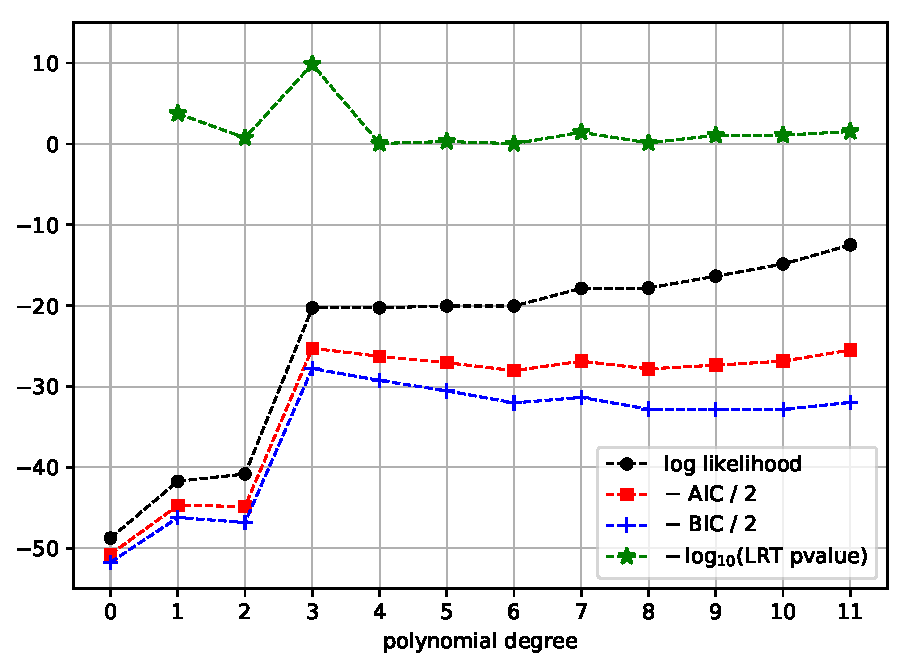
\includegraphics[width=0.60\textwidth]{./figs/03-linear-regression-LL-AIC-BIC-pvalue.pdf}
\end{figure}


\newpage
\no We can (approximately) calculate the probability that each model is correct.
\begin{itemize}
\item Using the BIC, the model evidence is $P(D\;|\;M_k) \approx e^{-\text{BIC}_k/2} / \sum_{k'=0}^Ke^{-\text{BIC}_{k'}/2}$
\begin{lstlisting}[language=python]
def BIC_weigths(BICs):
	BICs = np.array(BICs)
	w = BICs - np.min(BICs)  # to avoid underflow in the next line
	w = np.exp(-0.5*(w))  
	w /= np.sum(w)
	return w
\end{lstlisting}
\end{itemize}

\no Comparing the probabilities visually tells us a lot about the plausibility of the different models. We can see that models $M_0, M_1$ and $M_2$ have no chance, $M_3$ has the highest chance of being correct ($\sim 73\%$), while $M_4$ and $M_5$ are still possible, albeit with lower probabilities, $\sim 17\%$ and $\sim 5\%$, respectively.
\begin{figure}[h]
	\centering
	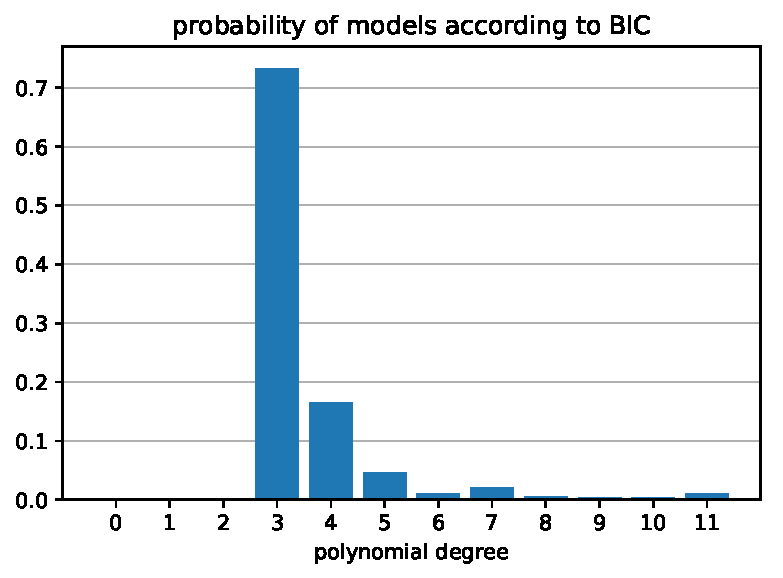
\includegraphics[width=0.7\textwidth]{./figs/03-linear-regression-BIC-weights.pdf}
\end{figure}


